\documentclass[12pt,a4paper]{report}

\usepackage[utf8]{inputenc}
\usepackage{amsmath}
%\usepackage{biblatex}


\usepackage{acronym}
\usepackage{amsfonts}
\usepackage{acronym}
\usepackage{amssymb}
\usepackage{graphicx}
\usepackage{chngcntr}
\usepackage{hyperref}
\usepackage[table]{xcolor}
\usepackage{glossaries}
\usepackage{caption}
\usepackage{booktabs}
\usepackage{algorithm}
\usepackage{subcaption}
\usepackage[hidelinks]{hyperref}%\usepackage{hyphenat}
\usepackage{titletoc}
\usepackage{tocloft}
\usepackage{pgfkeys} 
\usepackage{listings}
\usepackage[english]{babel}

\usepackage[
backend=biber,style=ieee]{biblatex}

\addbibresource{bibilo.bib}
\newcommand*{\bibtitle}{REFERENCES}



\usepackage{ragged2e}
\usepackage{setspace} \doublespacing
\usepackage[export]{adjustbox}
\usepackage{enumerate}
\usepackage[left=1in,right=0.9in,top=1in,bottom=1in]{geometry}
%\usepackage{lineno}
%\usepackage{cite}	
%\usepackage{acronym}
\renewcommand{\baselinestretch}{1.5}
\usepackage[utf8]{inputenc}
\usepackage[dvipsnames]{xcolor}
\usepackage{tikz} 
\usepackage{pgfgantt}

%-----------------for lof 
%\setlength{\cftfigaftersnum}{\hspace{10pt}}
%setmainfont{Times New Roman}
\usetikzlibrary{
	arrows,	calc,shapes,arrows,shapes.misc,shapes.arrows,chains,	matrix, 	positioning, scopes,	decorations.pathmorphing,	shadows, plothandlers,scopes,shapes.symbols,fit
}
\tikzstyle{startstop} = [ellipse, , minimum width=4cm, minimum height=1.2cm,text centered, draw=black,text width=3cm , rounded corners=0.5cm]
\tikzstyle{io} = [trapezium, trapezium left angle=70, trapezium right angle=110, minimum width=3cm, minimum height=1.2cm, text centered, draw=black,text width=3cm]
\tikzstyle{process} = [rectangle, minimum width=8cm, minimum height=1.2cm, text centered, draw=black  ]
\tikzstyle{process1} = [rectangle, minimum width=4cm, minimum height=1.2cm, text centered, draw=black  ]
\tikzstyle{decision} = [diamond, minimum width=7cm, minimum height=1.2cm, text centered, draw=black,aspect=2  ]


\tikzstyle{nodemcu} = [rectangle, minimum width= 3cm, minimum height= 10cm, text centered, draw = black, text width = 3cm]
\tikzstyle{blynkcloud} = [rectangle, minimum width= 3.5cm, minimum height= 7cm, text centered, draw = black, text width = 3cm]
\tikzstyle{sensor} = [rectangle, minimum width= 3cm, minimum height= 2cm, text centered, draw = black, text width = 2cm]
\tikzstyle{sensor1} = [rectangle, minimum width= 3cm, minimum height= 1cm, text centered, draw = black, text width = 2cm]

\usepackage{amsmath}
\usepackage{relsize}
\renewcommand{\cftfigfont}{Figure~}
\usepackage{tabularx}
\usepackage{multicol}
\usepackage{multirow}



\usepackage{sectsty}
\chaptertitlefont{\Large}
\sectionfont{\large}
\subsectionfont{\large}
\subsubsectionfont{\normalsize}
\paragraphfont{\normalsize}
\subparagraphfont{\normalsize}



\makeatletter
%\usepackage{titlesec}  
\usepackage[compact]{titlesec}  
\usepackage{times}
%\makeglossaries





\titlespacing*{\subsection}{0pt}{1.5 pt}{5pt}{ \fontfamily{times}}

\titleformat*{\subsubsection}{\centering \fontfamily{times}}
\titlespacing*{\chapter}{-2pt}{-20pt}{20pt}{ \fontfamily{times}}
\titlespacing{\section}{-2pt}{18pt}{5pt}{ \fontfamily{times}}


\titleformat{\chapter}[display]
{\normalfont\fontsize{16pt}{1.5pt}\selectfont\bfseries}{\chaptertitlename\ \thechapter}{0.5em}{\fontsize{16}{1.5pt}\selectfont\bfseries}

% Customize section headings
\titleformat{\section}
{\normalfont\fontsize{14pt}{1.5pt}\selectfont\bfseries}{\thesection}{0.5 em}{}

% Customize subsection headings
\titleformat{\subsection}
{\normalfont\fontsize{13pt}{2.5pt}\selectfont\bfseries}{\thesubsection}{0.5em}{}

\captionsetup{skip=0pt}
\setlength{\belowcaptionskip}{0pt}

%\setglossarystyle{list}
%\makeglossaries



%\newacronym{BMS}{BMS}{Battery Management System}
%\newacronym{CNC}{CNC}{Computer Numerical Control}
%\newacronym{DC}{DC}{Direct Current}
%\newacronym {GPRS}{GPRS}{General Packet Radio Service}
%\newacronym{GSM}{GSM}{Global System for Mobile Communications}
%\newacronym{HVAC}{HVAC}{Heating, Ventilation, and Air Conditioning}
%\newacronym {IDE}{IDE}{Integrated Development Environment}
%\newacronym{LDR}{LDR}{Light Dependent Resistor}
%\newacronym {LED}{LED}{Light Emitting Diode}
%\newacronym{MHz}{MHz}{Mega Hertz}
%\newacronym{MQ2}{MQ2}{Metal Oxide Semiconductor Type Gas Sensor}
%\newacronym{PCB}{PCB}{Printed Circuit Board}   	
%\newacronym{PIR}{PIR}{Passive infrared }
%\newacronym{PWM}{PWM}{Pulse Width Modulation}
%\newacronym{RFID}{RFID}{Radio Frequency Identification}
%\newacronym{RV}{RV}{Rotary Vane}
%\newacronym{SMS}{SMS}{Short Message Service}
%\newacronym{USB}{USB}{Universal Serial Bus}
%\newacronym{VSM}{VSM}{Value Stream Mapping}
%\newacronym{Wi-Fi}{Wi-Fi}{Wireless Fidelity}


%\newglossarystyle{custom_acronyms}{%
	%	\setglossarystyle{long}% Use the long style as the base
	%	\renewenvironment{theglossary}{\begin{enumerate}[itemsep=12pt]}{\end{enumerate}}% Adjust spacing between items
	%}






\begin{document}
	
	%------------------------------------Title Page--------------------------------------------------------	
	\begin{center}
		\large{
			\textbf{ \Large {KANTIPUR ENGINEERING COLLEGE} \\}
			\textbf{ (Affiliated to Tribhuvan University)\\ Dhapakhel, Lalitpur \\}
			
			
			\vfill
			
\includegraphics[width=0.3\textwidth]{images//logo.png} \\
			
			\vfill
			\textbf{[Subject Code: EX 654]}
			\vfill
			\textbf{ A FINAL MINOR PROJECT  REPORT \\ ON\\ \large{``HOME AUTOMATION''} }
			
			\vfill
			
			
			\begin{tabular}{l l}
				\textbf{Prakriti Thapa} &  \textbf{[33320]} \\
				\textbf{Pratap Niraula} & \textbf{[33321]} \\
				\textbf{Sabin Thapa Magar} & \textbf{[33324]} \\
				\textbf{Sunil Bahadur Singh} & \textbf{[33331] }
				
			\end{tabular}
			
			
			
			
			\vfill
			
			
			\textbf{Submitted to:\\
				Department of Computer and Electronics Engineering\\
				\vfill
				February, 2024
			}
		}
	\end{center}
	\pagenumbering{gobble}
	
	%---------------------------------Abstract Page --------------------------------------------------	
	
	\pagebreak
	\addtocontents{toc}{\protect\setlength{\cftbeforechapskip}{-10pt}} % Adjust the value as needed
	\addcontentsline {toc} {chapter} {Abstract}
	\thispagestyle{plain}
	
	\begin{center}
		\textbf{\fontsize{16}{1.5pt}\selectfont ABSTRACT}
	\end{center}
	
	
	\begin{justify}
		With an exponential advancement of automation technology, the future of manual systems are changing into automatic systems for various benefits. Home automation is one of the application of these advancement. This  field of automating living places is continuously arising making house safer and better place to live. Home Automation project is designed to revolutionize traditional home by integrating IOT based home automation system using ESP32 module. These system encompass bulb control, door lock security, kitchen fire protection ,and tank water management with various sensors strategically placed throughout the home. PIR and LDR is used for Light control, RFID is used for door lock security, MQ2 and Water level sensor is used for kitchen fire protection and tank water management system respectively.  The system will automatically control appliances on the basis of sensors data by constantly monitoring the home environment and storing sensors data onto the cloud.   
		Users can  also monitor and control this system using Arduino IoT cloud platform.\\
		
		
		\textbf{Keywords:} \textit { ESP32, IoT, MQ2, PIR, RFID, Water level sensor }
		
	\end{justify}
	\pagenumbering{roman}
	
	
	%----------------------ACKNOWLEDGEMENT------------------------------------------------------------------------------
	\pagebreak
	\addtocontents{toc}{\protect\setlength{\cftbeforechapskip}{0pt}}
	\addcontentsline {toc} {chapter} {Acknowledgement}
	\thispagestyle{plain}
	
	\begin{center}
		
		\textbf{\fontsize{16}{1.5pt}\selectfont ACKNOWLEDGEMENT}
	\end{center}
	
	
	\begin{justify}
		We are writing to express our sincere gratitude to the \textbf{ Department of Computer and Electronics Engineering,Kantipur Engineering College}  for providing us this  environment to initiate  minor project successfully. 
	\end{justify}
	
	\begin{justify}
		%second paragraph for 
		It is our great fortune that we have gotten an opportunity under the supervision of our Head of Department Er. Rabindra Khati sir, Deputy Head of Department Er. Anup KC sir and our project coordinator Er. Sujin Gwachha. The role of the respected teachers that have been with us through the times and have imparted invaluable knowledge, skill, understanding and wisdom is of undeniable importance.
		
		
	\end{justify}
	
	
	
	
	\begin{FlushLeft}
		\textbf{Group Members:}	 \\
		Prakriti Thapa \\
		Pratap Niraula \\
		Sabin Thapa Magar \\
		Sunil Bahadur Singh 
	\end{FlushLeft}
	
	
	%---------------------------------------------TABLE OF CONTENTS  ------------------------------------------
	%----------------------------------------------------------------------------------------------
	%-----------------------------------------------------------------------------------------------
	\pagebreak
	\thispagestyle{empty}
	\addcontentsline {toc} {chapter} {Table of contents}
	
	
	% Remove page number and header from the table of contents
	\begin{center}
		
		
		\setlength{\cftbeforetoctitleskip}{-13pt}
		
		\renewcommand{\contentsname}{\fontsize{16pt}{1.5pt}\selectfont\bfseries\textbf{TABLE OF CONTENTS} \fontfamily{times}}
		\setlength{\cftaftertoctitleskip}{2pt}
		\tableofcontents
	\end{center}
	
	
	
	
	
	%---------------------------------------------------------List of Figures---------------------------------------------
	
	\pagebreak
	
	
	
	\addcontentsline {toc} {chapter} {List of figures}
	\thispagestyle{plain}
	
	
	
	
	
	\begin{center}
		\setlength{\cftbeforeloftitleskip}{-15pt}
		
		\renewcommand{\listfigurename}{\fontsize{16}{1.5}\selectfont\bfseries\textbf{LIST OF FIGURES}}
		%	\setlength{\cftbeforefigskip}{0pt}
		\setlength{\cftafterloftitleskip}{1.5pt}
		\listoffigures 
	\end{center}
	
	
	%-------------------------------------------------------------------------List of Tables---------------------------------------------------
	\pagebreak
	\addcontentsline {toc} {chapter} {List of tables}
	\thispagestyle{plain}
	\begin{center}
		\setlength{\cftbeforelottitleskip}{-15pt}
		\renewcommand{\listtablename}{\fontsize{16}{1.5}\selectfont\bfseries\textbf{LIST OF TABLES}}
		\setlength{\cftafterlottitleskip}{1.5pt}
		\counterwithin{table}{chapter}
		
		\renewcommand{\cfttabpresnum}{Table\space}
		\cftsetindents{table}{0em}{4.5em}
		\listoftables
	\end{center}
	
	
	
	
	%----------------------------------------------------GLossary of Acronyms---------------------------------------------
	\pagebreak
	\addcontentsline {toc} {chapter} {Abbreviations}
	\thispagestyle{plain}
	\begin{center}
		\textbf	{\Large {ABBREVIATIONS} \\}
	\end{center}
	
	
	\vspace{0.1cm}
	%	\glsaddallunused % Include all abbreviations even if not explicitly used in the document
	%	\printglossary[title={}, type=\acronymtype, style=myalttree]
	\begin{justify}
		\begin{tabular}{l l}
		
			ADC & Analog to Digital Conveter \\
			ESP32 & Espressif System 32\\
			GPIO & General Purpose Input Output \\
			IDE & Integrated Development Environment\\
			IoT & Internet of Things \\	
			LDR & Light Dependent Resistor\\
			LED & Light Emitting Diode\\
			MHz &Mega Hertz\\
			MQ2 & Metal Oxide Semiconductor Type Gas Sensor\\
			PCB & Printed Circuit Board\\
			PIR & Passive infrared \\
			PWM & Pulse Width Modulation\\
			RFID & Radio Frequency Identification\\
			SMS & Short Message Service\\
			USB & Universal Serial Bus\\
			VSM & Value Stream Mapping\\
			Wi-Fi & Wireless Fidelity 
		
			
		\end{tabular}
		
		
		
	\end{justify}
	
	
	
	% Print the acronym list
	
	
	
	
	%	\printacronyms
	
	
	
	%------------------------------------------------------Chapter 1 Introduction ---------------------------------------------
	
	\chapter{INTRODUCTION}
	\addtocontents{toc}{\protect\setlength{\cftbeforechapskip}{16.5pt}}
	\pagenumbering{arabic}
	
	\section{Background}
	
	\begin{justify}
		Home automation, smart home automation system is a means that enable individuals to control electric appliances smartly and automatically within a home environment to make life easy by providing convenience, comfort, security  and energy efficiency to its inhabitants.[1]   These systems are designed to automate tasks and functions that were traditionally performed manually. Different household appliances like light, door, fan, heater, etc is controlled and monitored to provide home automation and security.Sensors can monitor changes in daylight, temperature, or motion detection. Home automation systems can then adjust those settings and also more to own preferences. Actuators are light switches, motors, or motorized valves that control the actual mechanism, or function, of a home automation system. They are programmed to be activated by a remote command from a controller.
	\end{justify}
	\begin{justify}
		This home automation system exits from many years. Home automation systems represents a great research opportunity in creating new fields in engineering, and computing.[2] Home automation and security system includes centralized control of lightning, monitoring and many more. But we focused this project for the security based home automation system of gates and doors and other system. It can also help protect your home from disaster. It is becoming popular nowadays and enter quickly in this emerging market. However, end users,especially the disabled and elderly due to their complexity and cost,do not accept these systems.
		
	\end{justify}
	
	\begin{justify}
		Talking about the system, this system is proposed to control and examine this overall house mechanism in easier and convenient way. Temperature, Fire, Water level, etc are examined by this system and then appropriate task or output is implemented.
	\end{justify}
	
	%---------------------------------------------------------------------Problem Statement--------------------------------------------------------------------
	
	\section{Problem Statement}
	
	\begin{justify}
		In majority of the houses we see the tank water over flowing. It results in waste of water as well as electricity, so the concept of automatic water pump was established. Gas cylinder hazards have been encountered as prime reasons for loss in life and property. In order to solve such situation switches and fire alarm messages was introduced. While the sensor detects the fire near the gas cylinder,the servo lock closes the regulator and alert will send to the house owner. For security reasons, radio waves tag and reader is very strong, that's why RFID controlled door unlock system was introduced. Nowadays automation is preferred in the world which saves time and money in various ways and time is very precious. IoT based system is also introduced to monitor and control  house regardless the distance. In overall, there is a need of a system that can automate household tasks which improves the quality of life and saves power. 
	\end{justify}
	
	%	----------------------------------------------------------------Objective-------------------------------------------------------------------
	\section{Objective}
	
	\raggedright
	{ The main objectives of this project are: \\
		\begin{itemize}
			%	\setlength\itemsep{0.5em}
			\setstretch{1}
			
			\item  To implement IoT for device control using Arduino IoT cloud.
			\item To provide comfort and convenience to consumers and maintain safety in the house from fire and thief.
		\end{itemize}
	}
	
	%--------------------------------------------------------------Application------------------------------------------------------------------
	\section{Application}
	
	\begin{justify}
		Home automation systems can be used in various settings beyond residential homes. They offer convenience, efficiency, and enhanced control over devices and systems, making them suitable for a wide range of applications.\\Home automation can be employed in offices, hotels, restaurants, and other commercial establishments to regulate lighting, and security, optimizing energy consumption and enhancing user comfort. Schools and universities can benefit from automation systems to manage lighting and security within classrooms, libraries, and other areas. Home automation can be adapted for healthcare settings to control lighting, temperature and gases leakage. It can also be used for patient monitoring and to improve accessibility for patients with disabilities.Home automation systems can be employed in remote locations, such as wildlife monitoring stations..
	\end{justify}
	
	
	%--------------------------------------------------------------Project Features------------------------------------------------------------------
	\section{Features}
	
	\raggedright
	{ Some features of this project are: \\
		\begin{itemize}
			\setstretch{1}
			%	\setlength\itemsep{0.5em}
			\item  RFID system door unlocking, Sends alert when unknown person is detected.
			\item  Turn lights on/off according to motion detected.
			\item  Automatically fills the tank without spillage.
			\item Detect the presence of fire or flame an turn off the regulator by servo, turns all the power supply off of the kitchen. 
			
			
		\end{itemize}
	}
	
	%-------------------------------------------------------------------Feasibility Analysis--------------------------------------------------------------------
	\section{Feasibility Analysis}
	
	\begin{justify}
		
		Feasibility analysis is a crucial step in evaluating the viability of a home automation project before proceeding with its implementation. It helps assess the project's practicality, cost-effectiveness, and potential benefits. Here are the key aspects to consider during a feasibility analysis of a home automation project: 
	\end{justify}
	
	\subsection{Operational Feasibility}
	
	\begin{justify}
		The system will be well documented and easy user interfaces will be implemented for the modules. This will ensure that the system can be easily handled and operated by the person. All the systems are worked on a different module so there is no chance of collision in a system. it requires minimum operational skills so it is user friendly and easy to use.
	\end{justify}
	
	\subsection{Economic Feasibility}
	
	\begin{justify}
		The project can be built in a low price as compared to the features it can provide. All the components are easily available in Local Electronics Market ans well as in our college in reasonable cost. Overall, the project prototype is feasible enough for a residential home and implementation is also feasible.
	\end{justify}
	
	\subsection{Technical Feasibility}
	
	\begin{justify}
		The system consists of easily available electronic components like Node MCU, Water level sensor, PIR sensor , RFID sensor, MQ2 sensor and easily available   data sheets. The component works in low voltage so there is no electrical risks. The programming tools and software like Arduino IDE are open source.
	\end{justify}
	
	%-----------------------------------------------------------------------------Literature Review ----------------------------------------------------------------------------------------------------
	\chapter{LITERATURE REVIEW}
	
	\section{Related work}
	\begin{justify}
		The system that automates home  has been designed and developed for a very long time now. The paper below has presented brief summaries of different past attempts which were made for developing systems related to home automation system using various technologies.
	\end{justify}
	
	
	\begin{justify}
		
		
		
		Customary homes to smart homes using internet of things (IoT) and mobile application by Govindraj,  Sathiyanarayanan, and Abubakar \cite{govindraj2017customary} presented a smart home automation system to replace the conventional home automation system using IoT technologies. The paper discussed use of  an Android application to control and monitor appliances, temperature, motion, and gases in the home environment, which is carried out via a satellite station and a radio frequency transceiver. Data generated by sensors are stored on the ThingSpeak cloud platform and can be monitored wirelessly.
	\end{justify}
	\begin{justify}
		Smart automated home application using IoT with Blynk app by Durani, Mitul, Vaghasia, and Kotech \cite{durani2018smart} based their home management system on IoT technologies and Blynk mobile.They controlled devices and multiple sensors in a house through the Internet. Their proposed system  designed to operate in both SMS  modes, via a phone, and an online mode, via a desktop computer. The proposed system incorporates sensors to monitor temperature and humidity and detects a fire, gas leakage, or intruders in the house.
	\end{justify}
	
	\begin{justify}
		
		
		Home Automation System Using Nodemcu (ESP8266) by Rajeshkumar, G and Rajesh Kanna, P and Sriram, S and Sadesh, S and Karunamoorthi, R and Mahudapathi, Prasad \cite{rajeshkumar2022home} implemented home  automation using ESP8266(Node MCU) along with PIR and LDR using andriod application by Blynk App page to use it remotely. This paper discussed about the use of these  devices wirelessly from anywhere using  Wi-Fi technology. 
	\end{justify}
	
	\begin{justify}
		The existing literature on home automation reveals notable research gaps that our project seeks to address. Poor home security and lack of emphasis on energy efficiency,   leading to potential wastage is observed in many paper. Our project addresses  by incorporating features to conserve energy resources, and  allowing users to monitor and control electronic devices fruitfully. Additionally, our project addresses the issue of IoT connection failure, ensuring that even in such scenarios, the automatic system can autonomously sense and carry out tasks seamlessly, enhancing the reliability and resilience of the home automation system.
		
		
	\end{justify}
	
	%------------------------------------------------------------------------------------------System Requirements--------------------------------------------------------------------------------------------
	\chapter{SYSTEM REQUIREMENTS}
	
	\section{Software Requirements}
	
	\begin{enumerate}
		\setstretch{1}
		
		\item  Proteus	
		\item  Arduino Software (IDE)
		\item Arduino IoT cloud
	\end{enumerate}
	\vspace{2 px}
	
	\subsection{Proteus}
	
	\begin{justify}
		Proteus is a comprehensive software suite  that serves as a powerful tool for electronic circuit design and simulation. It consists of two main modules: ISIS for schematic capture, allowing users to design circuits by placing components and connecting them with virtual wires, and ARES for PCB layout design, facilitating manual and automatic component placement and routing. Additionally, the Proteus VSM module enables real-time simulation of electronic circuits, allowing users to virtually test the behavior of components and microcontrollers.
	\end{justify}
	
	\subsection{Arduino Software (IDE)}
	
	\begin{justify}
		The Arduino IDE (Integrated Development Environment) is a software platform specifically designed for programming Arduino microcontroller boards. It provides a user-friendly interface that simplifies the process of writing, compiling, and uploading code to Arduino boards. The IDE is open-source and available for multiple operating systems, including Windows, macOS, and Linux. It uses a simplified version of the C++ programming language, making it accessible to beginners and experienced developers alike. The IDE also offers a serial monitor, allowing users to interact with their Arduino board and debug code by sending and receiving data in real-time. 
	\end{justify}


	
	\subsection{Arduino IoT cloud }
	
	\begin{justify}
		
	
Arduino IoT Cloud is a comprehensive platform that facilitates the development and management of Internet of Things (IoT) projects using Arduino devices and other 3rd party device such as ESP32. It provides a user-friendly environment for connecting Arduino boards to the cloud, enabling remote monitoring and control of IoT applications. With Arduino IoT Cloud, users can easily create and customize dashboards to visualize real-time data from their connected devices.Arduino IoT Cloud supports automation through "Things," which are essentially the connected devices. Users can create rules and automation logic based on triggers and actions, enhancing the autonomy of their IoT applications.
	\end{justify}
	
	
	
	
	
	%---------------------------------------Hardware Requirement ----------------------------------------------------------
	
	\section{Hardware Requirement}
	\vspace{4pt}
	\begin{enumerate}
		\setstretch{0.8}
		
		\item  ESP32
		\item  Servo Motors
		\item  RFID Sensor
		\item  LDR
		\item  PIR  Sensor
		\item  MQ2 Sensor
		\item Water Level Sensor
		\item Water Pump Motor
		
		
		
		

	\end{enumerate}
	\vspace{3px}
	\subsection{ESP 32}
	\begin{justify}
		The ESP32 is a series of low-cost, low-power system-on-a-chip (SoC) microcontrollers developed by Espressif Systems. It is a IoT platform and is affordable.  The ESP32 provides a number of GPIO (General Purpose Input/Output) pins that can be configured as digital input or output. It  has a built-in ADC (Analog-to-Digital Converter) that allows it to read analog signals. The firmware is also included. The firmware offers a straightforward programming environment that is extremely straightforward to script.The ESP32 integrates a Wi-Fi module, making it capable of connecting to Wi-Fi networks. The Wi-Fi capabilities make the ESP32 suitable for IoT applications where internet connectivity is required. 
		
		
	\end{justify}
	
	
	\begin{center}
		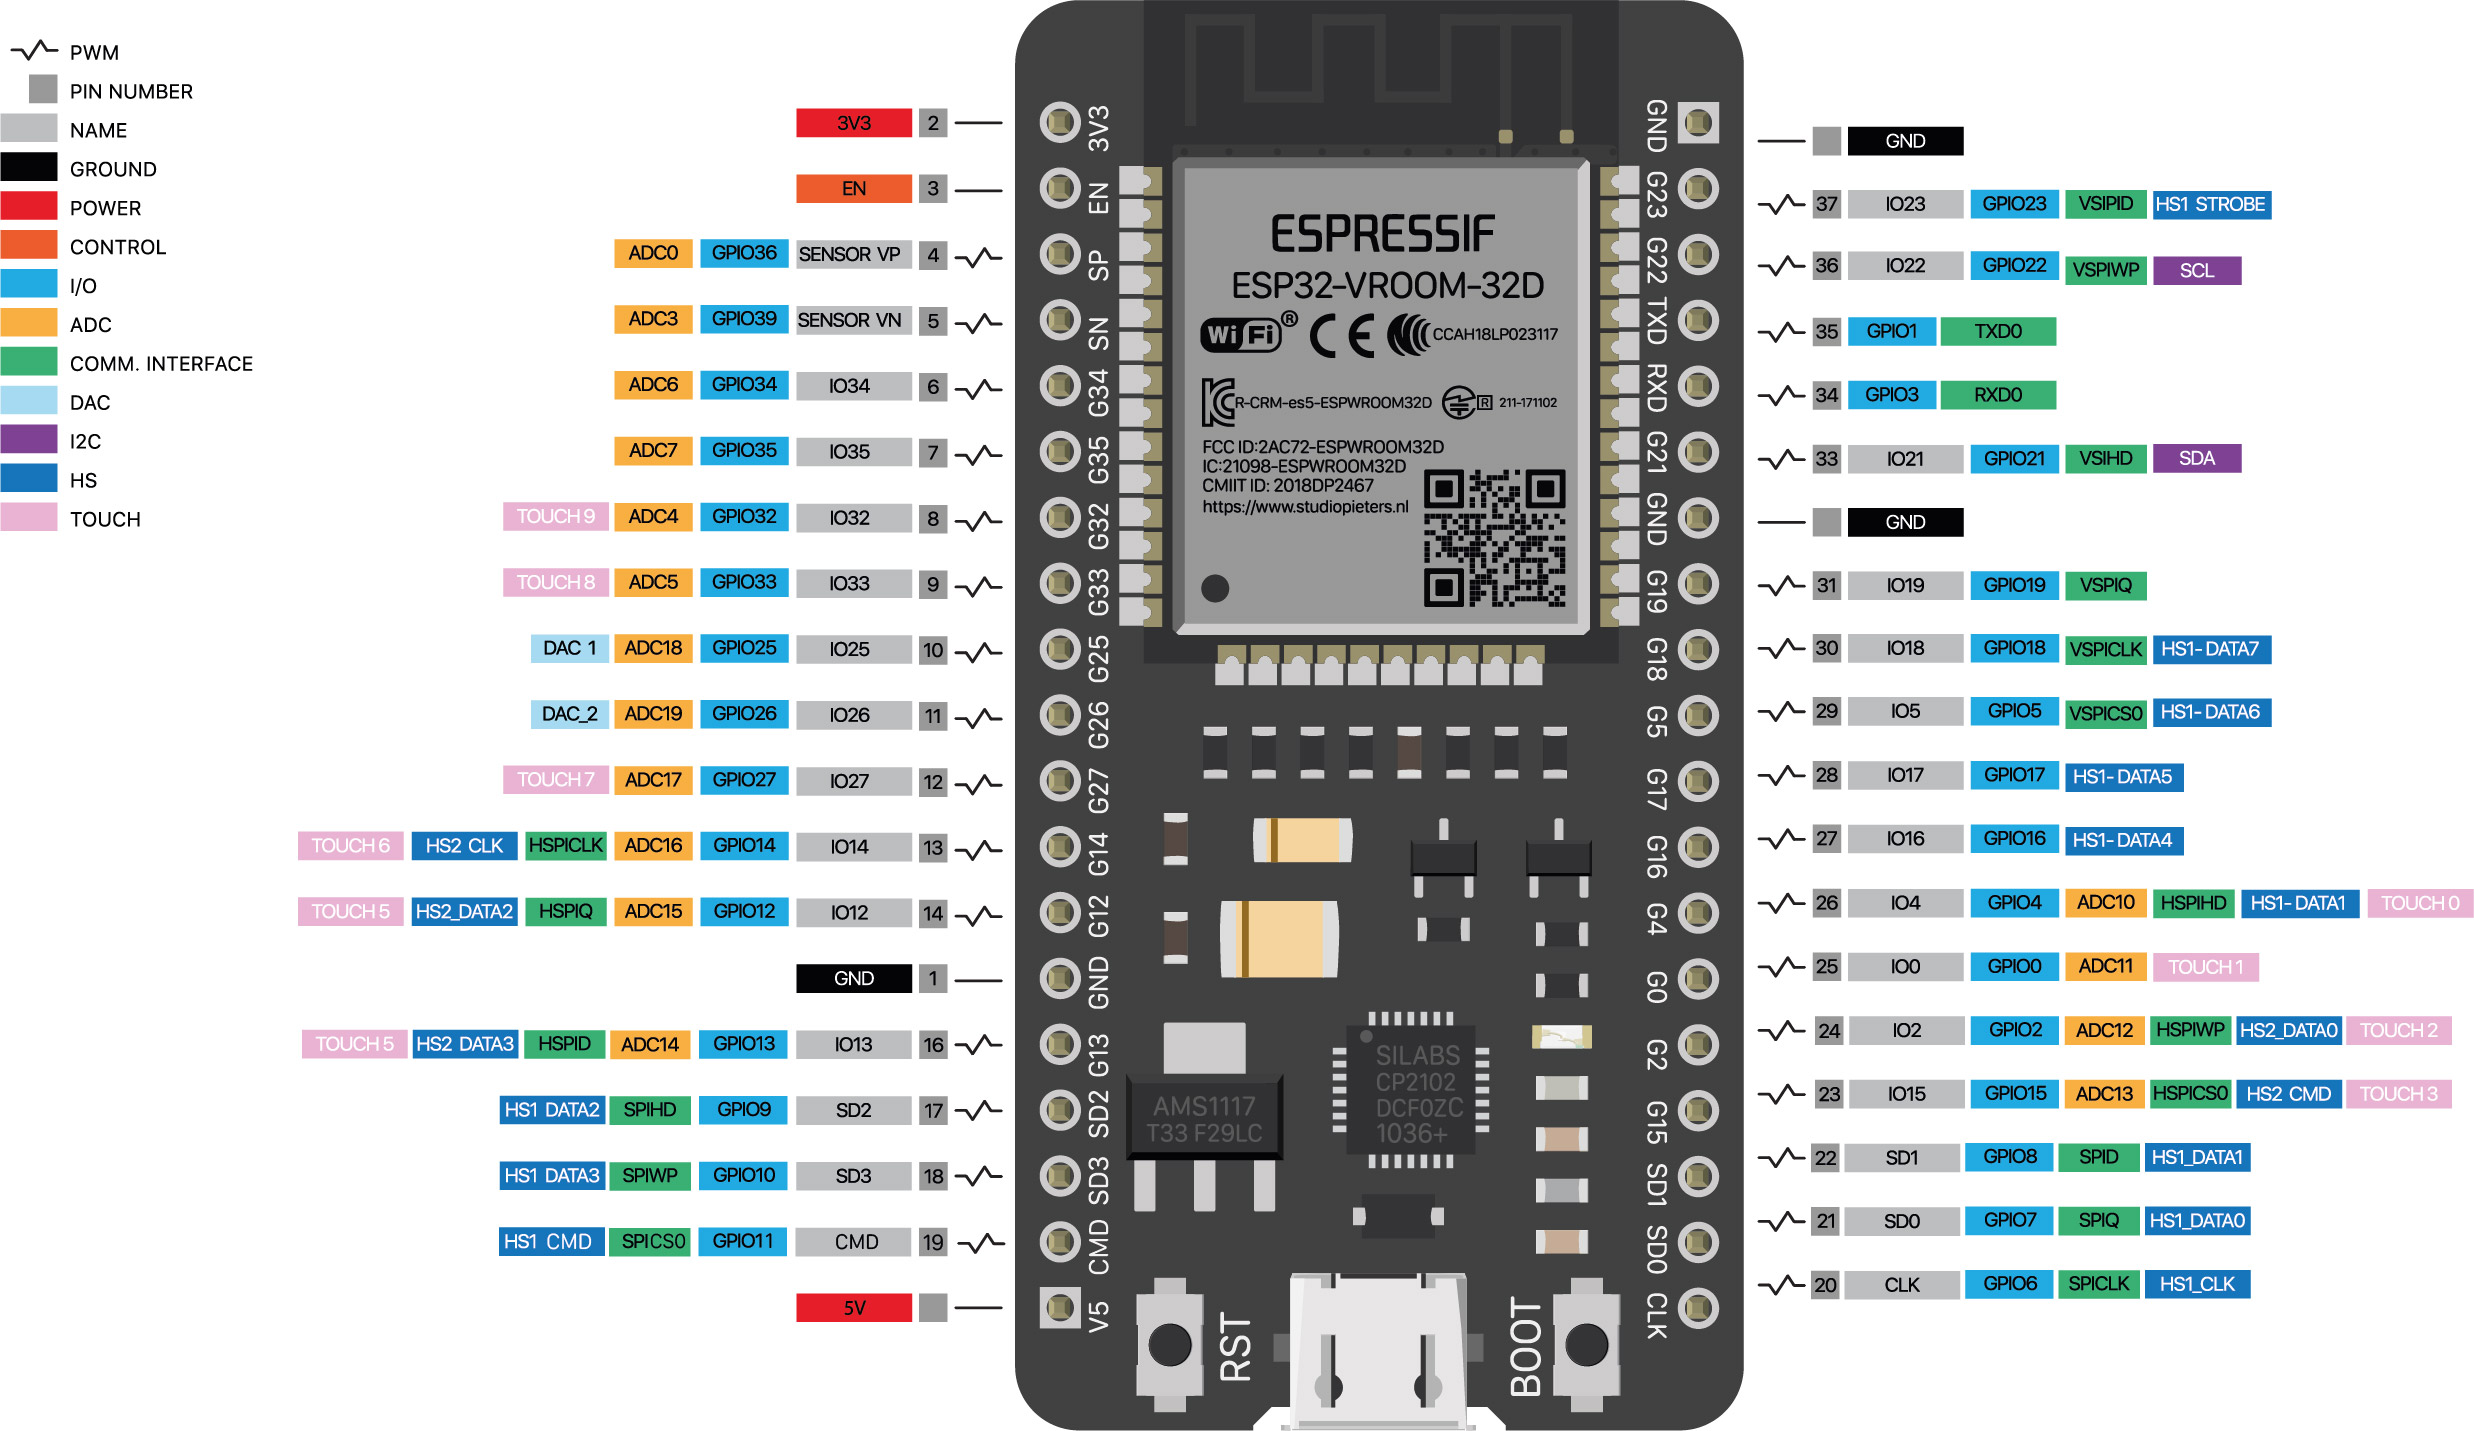
\includegraphics[width=0.5\textwidth]{images//esp.jpg}\\
		\begin{figure}[ht]
			
			\caption{ESP32 }
			\subsubsection{Source: (http://tinyurl.com/574w7wx6)}
			
		\end{figure}
		
	\end{center}
	
	
	\subsection{Servo Motors}
	\begin{justify}
		A servo motor is defined as an electric motor that allows for precise control of angular or linear position, speed, and torque. It consists of a suitable motor coupled to a sensor for position feedback and a controller that regulates the motor’s movement according to a desired setpoint. Servo motors consist of a DC motor, a gearbox, and a feedback control system that continuously monitors and adjusts the motor's shaft position. The feedback mechanism, typically in the form of a potentiometer or an encoder, ensures that the motor's actual position matches the desired position sent by the control system. By adjusting the input signal, the control system regulates the motor's rotation and maintains it at the desired position, providing high accuracy, stability, and repeatability. 
	\end{justify}
	
	\begin{center}
		
		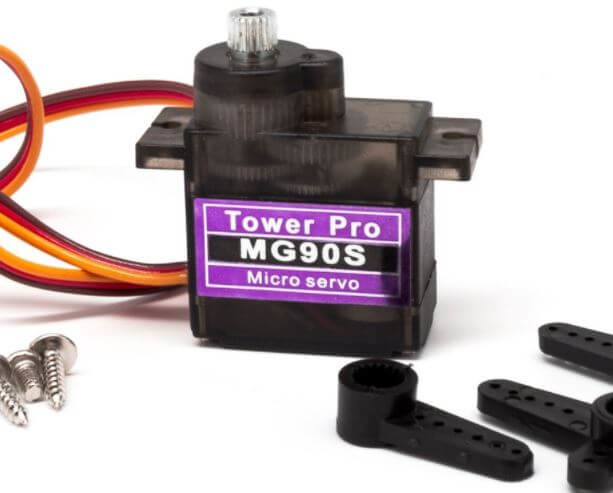
\includegraphics[width=0.32\textwidth]{images//servo_motor.jpg} 
		
		
		\begin{figure}[ht]
			
			
			\caption{Servo Motor}
			\subsubsection{Source: (http://tinyurl.com/mfp95738)}
		\end{figure}
		
	\end{center}
	
	
	%-------------------------------------

	
	\subsection{Water Pump Motor}
	\begin{justify}
		A 12-volt DC water pump motor is an electric motor specifically designed for driving water pumps. It is a critical component in water pumping systems, providing the necessary mechanical power to move water from one location to another. 12V water pump models are the standard operating motors for RV water pump, as these models are generally made for other purposes, generally in residential homes While 12V RV water pumps obviously don't pump water with the same pressure as larger ones made for installation in residential homes, but so long as they're in working order, they get the job done. It provides volume water flow with reduced pump cycling. These models are designed to run on water systems with no accumulator tank necessary, and up to five fixtures! It is also suited for use with a holding tank water system, as may be found in a boat, RV or remote cabin. It provides up to 5.0 gallons per minute. The water pumps are self-priming, and can run dry without damage, performance reliable and low current. This automatic demand water system pump has a relay switch, which automatically starts and stops the pump when the tank sensor is opened and closed.
	\end{justify}
	
	\begin{center}
		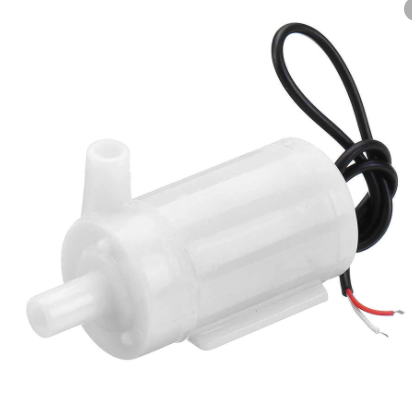
\includegraphics[width=0.31\textwidth]{images//water_pump.png} 
		
		\begin{figure}[ht]
			
			
			\caption{Water Pump Motor}
			
			\subsubsection{Source: (http://tinyurl.com/msb7uxfs)}
		\end{figure}
		
		
		
		
	\end{center}
	
	
	
	
	
	
	

	
	
	%-------------------------------------
	
	\subsection{PIR Sensor}
	\begin{justify}
		A PIR (Passive Infrared) sensor is a motion detection device that detects changes in infrared radiation emitted by objects within its field of view. It consists of a pyroelectric sensor, which is sensitive to infrared radiation, and a lens that focuses the infrared signals onto the sensor. PIR sensors work based on the principle that all objects with a temperature above absolute zero emit infrared radiation. When a person or an object moves in front of the sensor, the changes in the infrared radiation patterns are detected by the pyroelectric sensor, triggering an electrical signal. PIR sensors are commonly used in security systems, automatic lighting systems, and smart home devices to detect human presence and movement. Due to their passive nature they do not emit any radiation themselves. 
	\end{justify}
	
	\begin{center}
		
		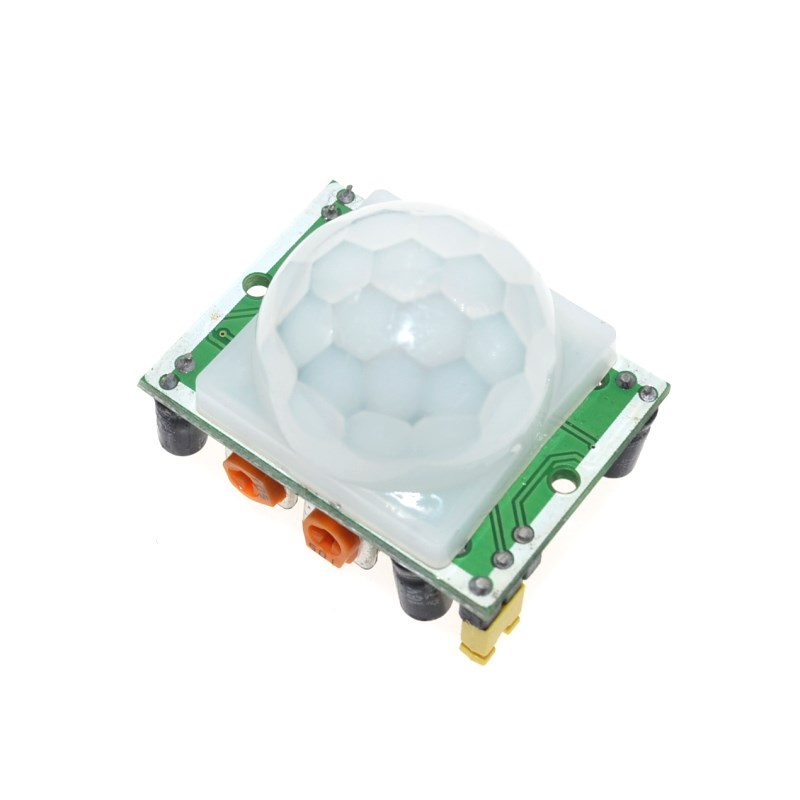
\includegraphics[width=0.3\textwidth]{images//pir_sensor.jpg}
		
		
		\begin{figure}[ht]
			
			
			\caption{PIR}
			
			\subsubsection{Source: (http://tinyurl.com/3k7ncvjk)}
		\end{figure}
		
	\end{center}
	
	%-------------------------------------
	
	
	
	\subsection{RFID Sensor}
	\begin{justify}
		An RFID  sensor is a technology that allows for the identification and tracking of objects or individuals using radio frequency signals. The RFID system consists of two main components: an RFID tag and an RFID reader or sensor. The RFID tag contains a unique identification code and an antenna, while the RFID reader emits radio frequency signals to communicate with the tag. When the RFID reader comes within range of the RFID tag, the tag's antenna captures the radio frequency signal, and it responds by transmitting its unique code back to the reader. The RFID sensor then decodes and processes this information, enabling the identification of the tagged object or person. RFID sensors are widely used in various applications, such as inventory management, access control systems, asset tracking, contactless payment systems, and electronic toll collection. 
	\end{justify}
	
	\begin{center}
		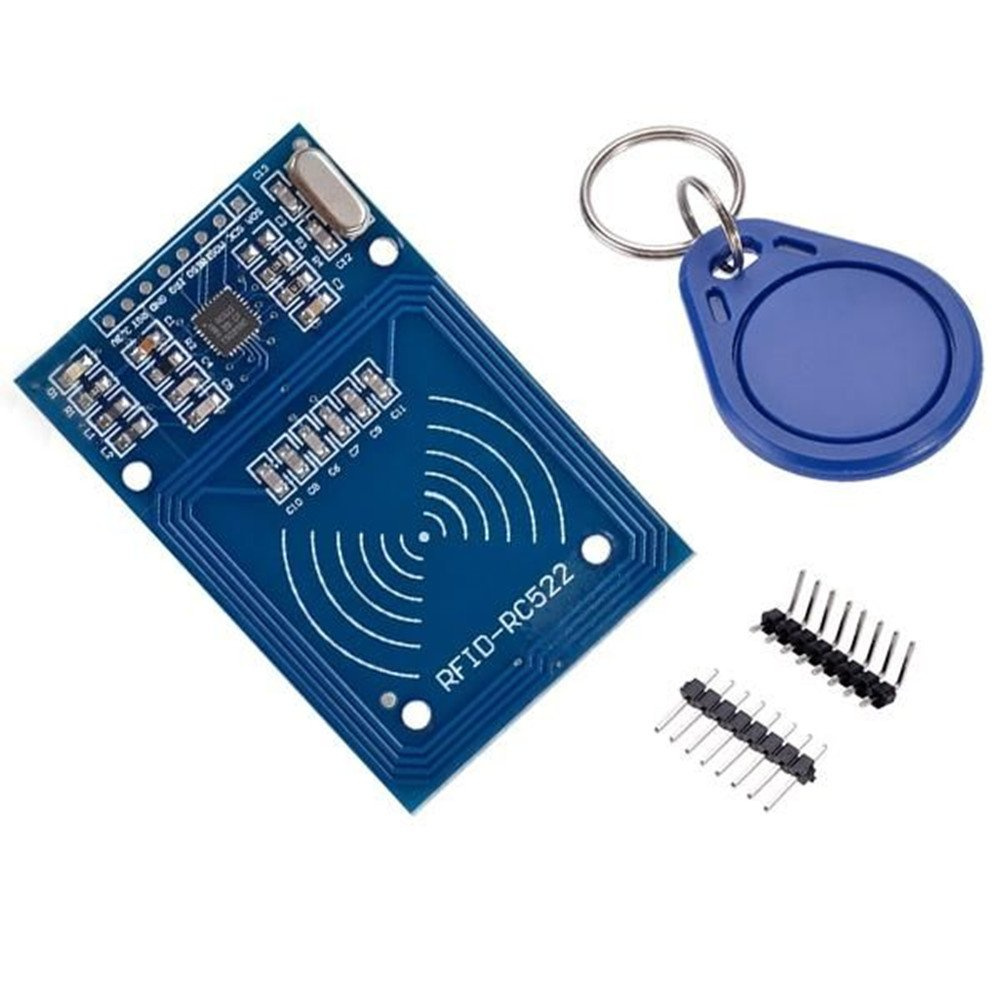
\includegraphics[width=0.4\textwidth]{images//rfid_sensor.jpg}  \\
		
		
		\begin{figure}[ht]
			
			
			\caption{RFID Sensor}
			
			\subsubsection{Source: (http://tinyurl.com/y6dy2yca)}
		\end{figure}
		
	\end{center}
	
	%-------------------------------------
	
	\subsection{LDR}
	
	\begin{justify}
		An LDR , also known as a photoresistor, is a type of semiconductor device that exhibits changes in its electrical resistance based on the intensity of light falling on it. The LDR is typically made of a high-resistance semiconductor material that becomes conductive when exposed to light. As the light intensity increases, the resistance of the LDR decreases, and vice versa. This unique property makes LDRs highly suitable for light sensing applications. In electronic circuits, LDRs are commonly used as sensors to detect ambient light levels, enabling automatic control of lighting systems. For example, LDRs can be employed in streetlights, indoor lamps, and camera exposure control, where they adjust the intensity of light output based on the surrounding light conditions. The sensitivity of LDRs can be fine-tuned by varying their physical properties or using additional circuitry.
	\end{justify}
	
	\begin{center}
		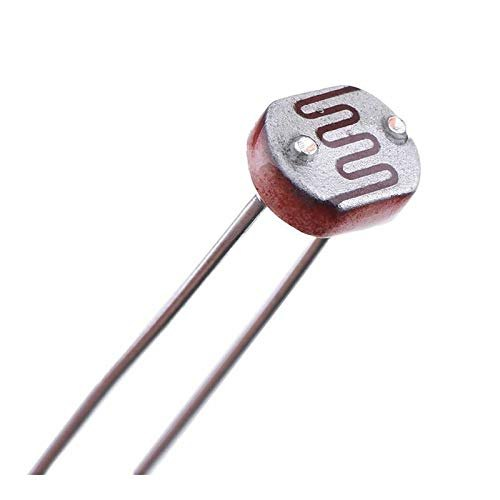
\includegraphics[width=0.22\textwidth]{images//ldr.jpg} \\
		
		\begin{figure}[ht]
			
			
			
			\caption{LDR}
			\label{fig:sample}
			\subsubsection{Source: (http://tinyurl.com/mr43xwpr)}
		\end{figure}
		
	\end{center}
	
	
	
	
	%-------------------------------------
	
	\subsection{Water Level Sensor}
	\begin{justify}A water level sensor is a device used to measure and monitor the depth of water in a tank, reservoir, or any other container. It provides valuable information about the water level, ensuring efficient water management and preventing overflows or shortages.The power and sense traces form a variable resistor (much like a potentiometer) whose resistance varies based on how much they are exposed to water.This resistance varies inversely with the depth of immersion of the sensor in water:The more water the sensor is immersed in, the better the conductivity and the lower the resistance.The less water the sensor is immersed in, the poorer the conductivity and the higher the resistance.
		
	\end{justify}
	
	\begin{center}
		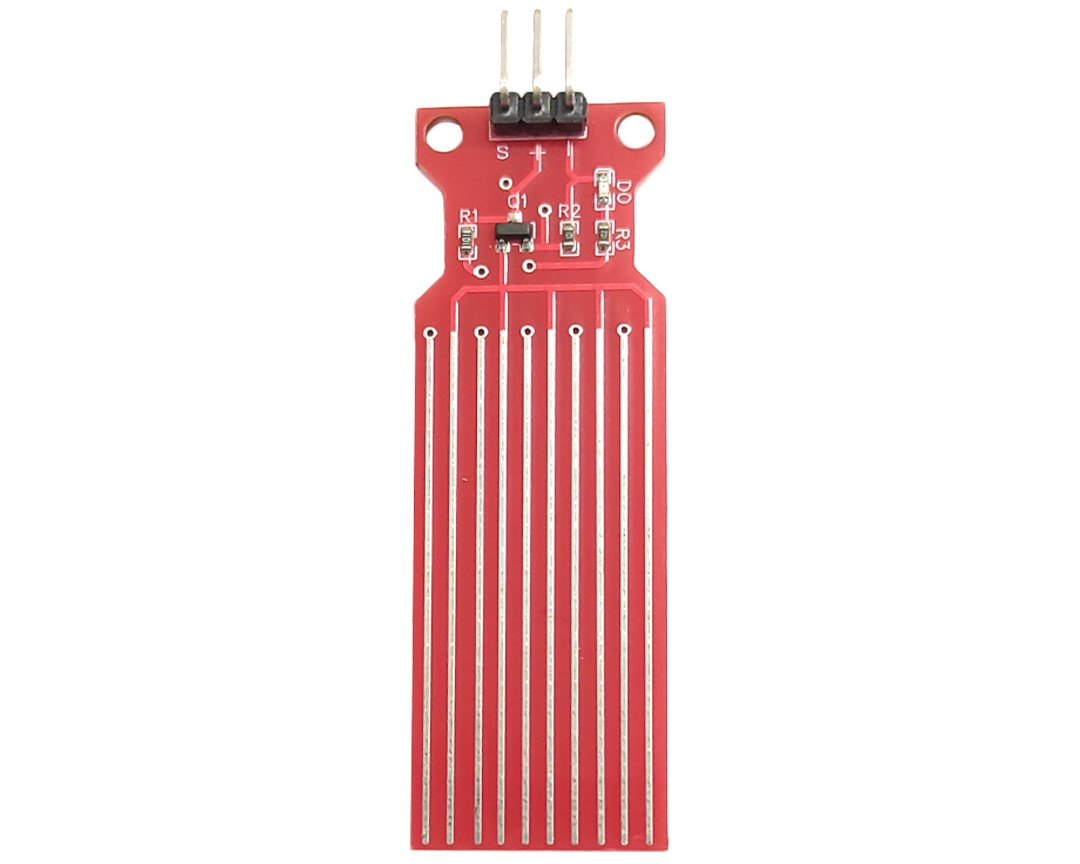
\includegraphics[width=0.48\textwidth]{images//waterlevel.jpg} 
		
		\begin{figure}[ht]
			
			\caption{Water Level Sensor}
			
		\end{figure}
		\vspace{-20pt}
		\subsubsection{Source: (http://tinyurl.com/3vh4e4tp)}
	\end{center}
	
	
	
	
	%-------------------------------------
	
	\subsection{MQ2 Gas Sensor }
	\begin{justify}
		The MQ2 gas sensor is a widely used semiconductor-based sensor designed to detect various combustible gases and smoke in the surrounding environment. It operates on the principle of gas absorption, where the presence of specific gases alters the sensor's conductivity, resulting in a change in its resistance. The MQ2 sensor is equipped with a heating element that increases the temperature of its sensitive layer. When the target gas or smoke comes into contact with the heated layer, the sensor's resistance changes, and this variation is measured to determine the gas concentration. It can detect gases like methane, butane, propane, alcohol, smoke, and other flammable gases, making it a valuable component in ensuring safety and early detection of potential hazards in various indoor and industrial environments. Its simplicity, low cost, and efficiency have made it a popular choice for gas detection applications.
	\end{justify}
	
	\begin{center}
		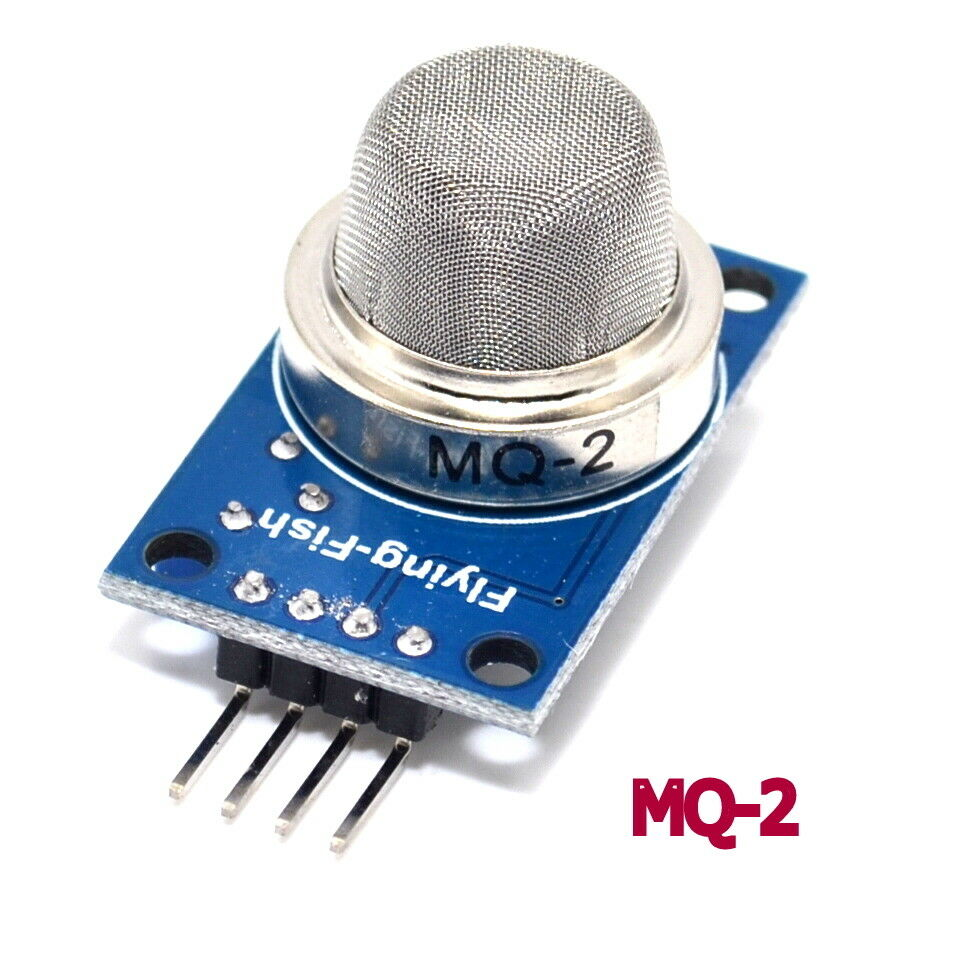
\includegraphics[width=0.3\textwidth]{images//mq2_gas_sensor.jpg} \\
		
		\begin{figure}[ht]
			
			
			\caption{MQ2 Gas Sensor}
			\label{MQ2 Gas Sensor}
		\end{figure}
		\vspace{-20pt}
		\subsubsection{Source: (http://tinyurl.com/3f9k5tk5)}
	\end{center}
	
	%-------------------------------------
	
	
	
	
	%-------------------------------------
	
	
	
	
	
	
	%-------------------------------------------------------chapter 4 methodology --------------------------------------------------------------------------------------
	\chapter{METHODOLOGY}
	
	\section{System Designs and Block Diagrams}
	
	%\begin{justify}
	%	In the below block diagram, the components are connected as required for Home Automation using IoT as shown. We connected all the sensors with Node MCU. We use Blynk Cloud and app to display data and control the sensors.We can control device and multiple sensors in house through the Internet using Blynk app. Node MCU ESP8266 microcontroller will read the data obtained from sensors like  \gls{PIR} sensor, \gls{RFID} sensor,etc and then it sends back signal to Blynk cloud.
	%\end{justify}\
	
	%----------------------------------------------------------------block diagram -----------------------------------------------------------------------
	
	
	\begin{Center}
		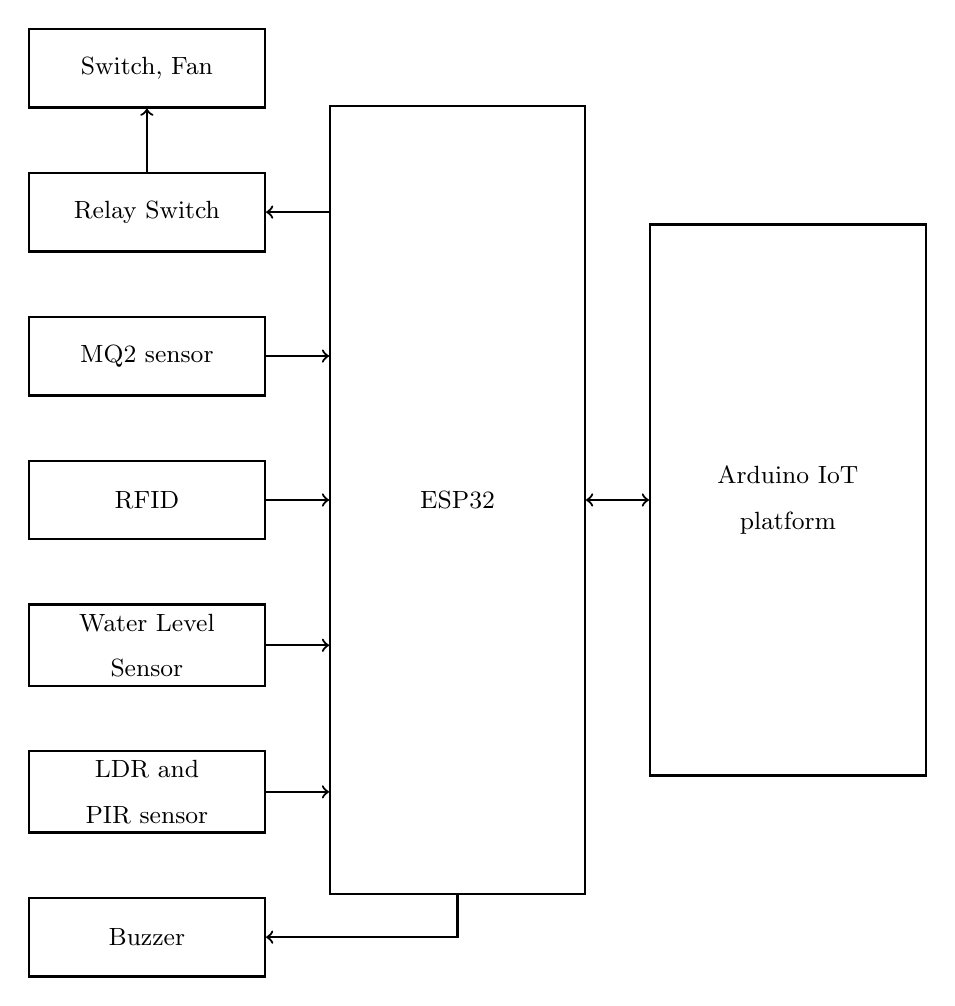
\begin{tikzpicture} [node distance=0.8cm]
			\tikzstyle{every node}=[font=\small]
			
			\node [blynkcloud, thick] (blynkcloud) at (0,0) {Arduino IoT platform} ;
			\node[nodemcu,  thick,  left  =  of blynkcloud] (nodemcu1){ESP32 };
			%	\node [nodemcu, below=of nodemcu1,thick] (nodemcu2) {ESP32 };
			
			\node[sensor1,  left =  of  nodemcu1, thick] (pir) { RFID};
			\node[sensor1, above = of  pir, thick] (MQ2) { MQ2 sensor};
			\node[sensor1, below = of  pir, thick] (watersensor) { Water Level Sensor};
			\node[sensor1, below =  of  watersensor, thick] (rfid) {LDR and PIR sensor};
			
			
			
			\node [sensor1, above=of MQ2, thick] (relay) {Relay Switch};
			\node [sensor1, below=of rfid, thick] (buzzer) {Buzzer};
			\node [sensor1, above=of relay, thick] (switch) {Switch, Fan};
			
			
			\draw[->,  thick] (pir) -- (nodemcu1.west);
			\draw[<->,  thick] (blynkcloud) -- (nodemcu1.east);
			\draw[<-,   thick] (relay.east) -- ++ (0.8cm,0);
			\draw[->,   thick] (relay.north) -- ++ (0,0.8cm);
			\draw[->,   thick] (MQ2.east) -- ++ (0.8cm,0);
			\draw[->,  thick] (rfid.east) -- ++(0.8cm,0);
			\draw[->,   thick] (watersensor.east) -- ++ (0.8cm,0);
			\draw[<-,   thick] (buzzer.east) -| (nodemcu1.south);
			
			%	\draw [<->, thick] (nodemcu2.north) -- (nodemcu1.south);
			%	\draw[<->,   thick] (nodemcu1.east) -- ++ (1cm,0);
			%	\draw[<->,   thick] (nodemcu2.east) -- ++ (1cm,0);	
			%	\draw[<->,  thick] (blynkcloud) -- (blynkapp.north);
			%\draw [->, thick] (blynkapp.west) -- ++ (-1cm,0) ;
			
		\end{tikzpicture}
		
		
		
		
		\begin{figure}[ht]
			
			
			\caption{Block Diagram}
			
		\end{figure}
	\end{Center}
	%---------------working of block diagram--------------
	\begin{justify}
		
		In the above block diagram, on the left side, various components such as sensors, switches, and a buzzer are present. The data from these sensors is sent  to the microcontroller ESP32. Upon receiving this data, the ESP32 facilitates relay, swtich, fan, buzzer, etc equipment according to logic used. The ESP32 continuously sends data to the  cloud, and this data can be monitored in the Blynk app. Using the Blynk cloud, we can control switches and devices like fans, enabling remote control functionality through ESP32.
	\end{justify}
	\begin{justify}
		
		Starting with sensors, we have use four main sensors; MQ2 sensor, PIR, RFID and Water level sensor.
		
	\end{justify}
	\begin{justify}
		
		
		The MQ2 gas sensor typically operates at a working voltage of 5V. This  gas sensing module capable of detecting various flammable and explosive gases, such as methane (CH4), propane (C3H8), butane (C4H10), LPG (Liquefied Petroleum Gas), and smoke in the air. It provides an analog output. The output value ranges from 0 -4095 values. WHen value from MQ2 sensor is read, it is send to the IoT platform. If the threshold value exceed  then  it indicates the presence of harmful gases. The exit fan is turned on  and Buzzer is turned on. Data from MQ2 sensor can be monitored from IoT platform.
	\end{justify}
	\begin{justify}
		The Water level sensor typically operates at a working voltage of 5V. It also  provides an analog output. Its working temperature is : 10℃~30℃.  This item can judge the water level through with a series of exposed parallel wires stitch to measure the water droplet/water size.  We use water level sensor for  Tank Water Management. Initially we set water pump motor off. Then we take data from level sensor. We send data to the IoT platform too. If the value is less than minimum threshold, we turn motor on and pump water and when the water level reach maximum of we turn off the motor and again constantly  read value from level sensor. 
	\end{justify}
	\begin{justify}
		
		PIR sensor operate in DC 4.5-20V. It provides digital output. We use PIR sensor with LDR sensor to work PIR only on night time. We read the value from LDR. If value is greater than  threshold, it indicate the night time. So we turn on PIR sensor and read value from PIR. If motion is detected then the blub glow in the room. We set delay time to turn off PIR and we again read value from PIR. if no any motion is detected we turn off PIR and take value from LDR. We can also turn on and off light through IoT platform.
	
	\end{justify}
	\begin{justify}
		
		RFID a technology that uses wireless communication to identify, track, and manage objects, people, or animals. RFID systems consist of tags (or transponders) and readers (or interrogators). The tags contain information that can be read by the readers using radio frequency signals. RFID sensor is use for door automation in our project. If the tag matches the RFID reader the door gets open. If the tag doesn't match the door won't get opened.
		
		
	\end{justify}\
	
	
	
	
	%----------------------------------------Block DIagram Explanation -----------------------------
	
	%{justify}
	%		Working of \gls{MQ2} Fire Sensor: \\ 
	%		\\The MQ2 gas sensor typically operates at a working voltage of 5V. It provides an analog output. The output value ranges from 0 -1023 values. This  gas sensing module capable of detecting various flammable and explosive gases, such as methane (CH4), propane (C3H8), butane (C4H10), LPG (Liquefied Petroleum Gas), and smoke in the air. Its threshold is around 400. After the threshold of 400 exceed, It indicates the presence of harmful gases.\\
	%     \\	Working of Water Level Sensor: \\ 
	%    \\The Water level sensor typically operates at a working voltage of 5V. It provides an analog output. The output value ranges from 0 -1023 values. Its working temperature is : 10℃~30℃.  This item can judge the water level through with a series of exposed parallel wires stitch to measure the water droplet/water size.Its minimum threshold value is 300 which indicate the tank is almost empty and the maximum threshold value is 520 that indicate the tank is almost full.\\
	%   \\Working of PIR sensor\\
	%  \\PIR sensor operate in DC 4.5-20V. We use PIR sensor with LDR sensor to work PIR only on night time. Firstly we connect PIR with cloud and observe the threshold value. If the threshold value is greater than 700 it indicate the absence of light  So, PIR sensor turn on if the motion is detected then the blub glow up. We can also control PIR from Blynk app to turn off and on the lights.\\
	% \\Working of RFID sensor \\
	%\\ RFID sensor is used for door automation. If the tag matches the RFID reader the door gets open. If the tag doesn't match for three times the door wont get open and lock for 3 minute.
	
	
	
	
	%\end{justify}
	
	
	
	
	
	%---------------------------------------------------------------flowchart----------------------------------------------------------------------------
	\pagebreak    
	\section{Algorithms and Flowcharts}
	\vspace{10pt}
	
	
	
	%----------------------------------------------------- FLowchart: Kitchen Room ------------------------------------------------------------------
	\subsection{Flowchart of MQ2 gas sensor for Kitchen Fire Protection}
	
	
	
	\begin{center}
		
		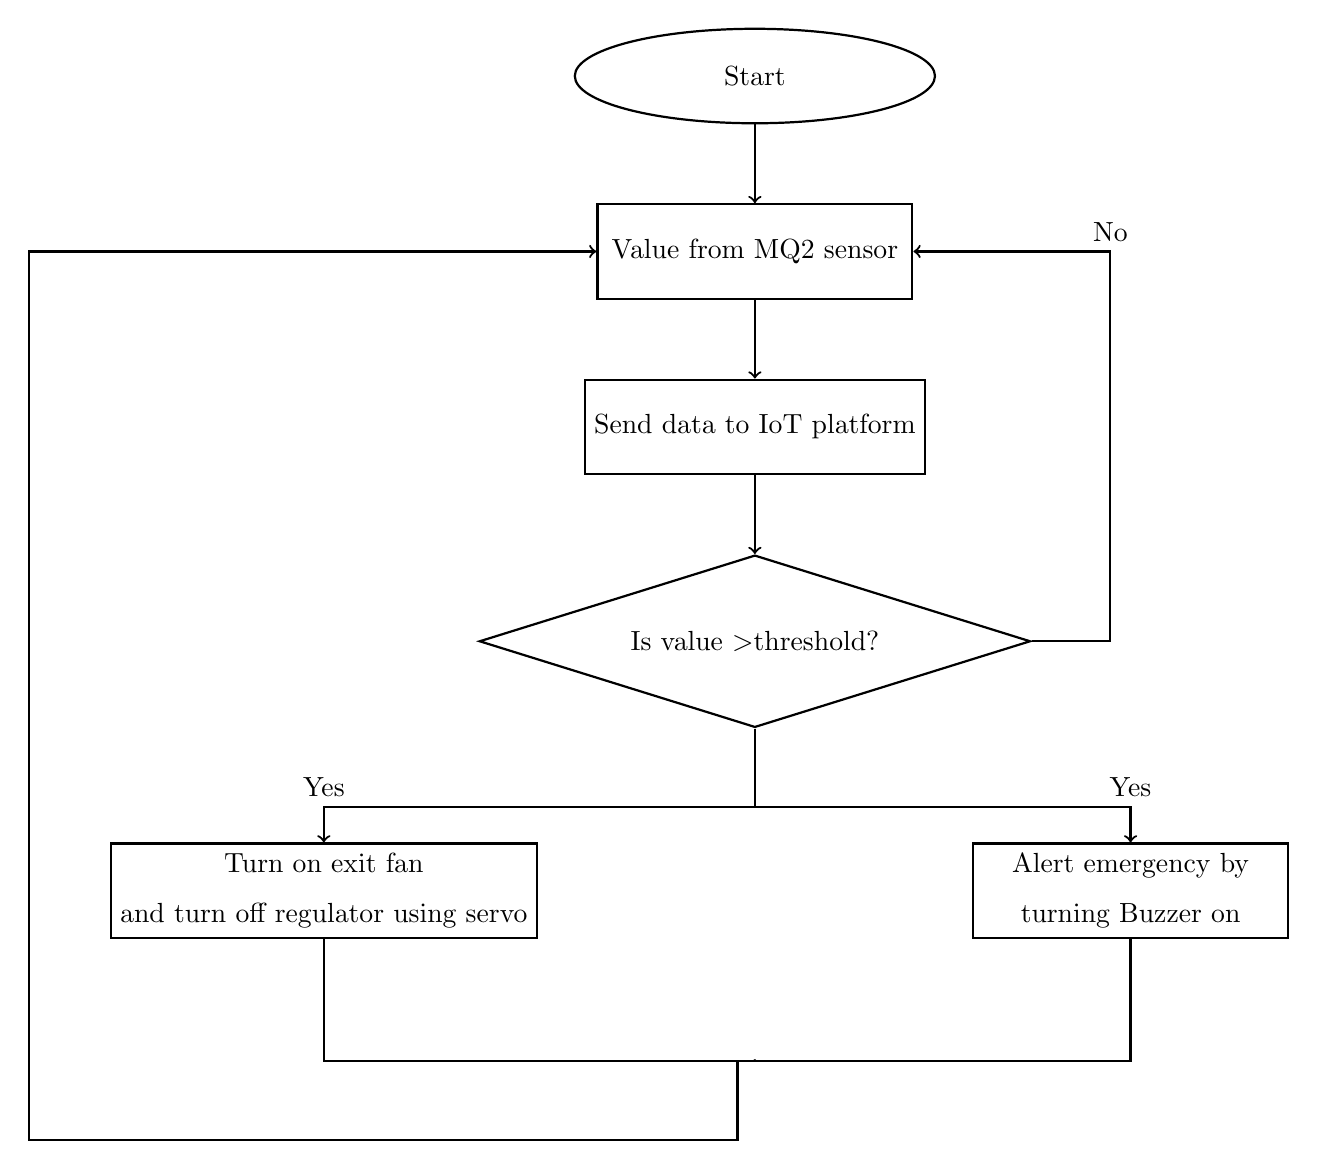
\begin{tikzpicture}  [node distance={1cm}]
			\node[startstop,  thick] (start){Start};
			
			\node[process1, below=of start,  thick] (proc1) {Value from MQ2 sensor};
			\node [process1, below=of proc1 ,thick] (cloud) {Send data to IoT platform};
			\node[decision, below=of cloud,  thick] (dec1){Is value \textgreater   threshold?};
			\node[process1, below left =2cm and 1cm of dec1,  thick, align=center] (proc2){Turn on exit fan \\ and turn off regulator using servo};
			\node[process1, below right = 2cm and 1cm of dec1,  thick, align=center] (proc3) {Alert emergency by \\turning Buzzer on };
			%	\node[process1, below left= 2.5cm and 2cm of dec1,  thick, align=center] (proc4){Cut Power Supply of \\ Kitchen  using relay };
			\node[circle,minimum size=0cm,below=4cm of dec1] (connector){.};
			%	\node[startstop,below= 4cm of dec1,  thick] (stop) {Stop};
			
			%arrow
			\draw [->,  thick] (start) -- (proc1);
			\draw [->,  thick] (cloud) -- (dec1);
			\draw [->,  thick] (proc1) -- (cloud);
			%	\draw [->,  thick] (dec1)  -- node[anchor=south] {Yes} (proc2);
			\draw [->,  thick] (dec1.east) -- ++(1,0)  |- node[anchor=south] {No} (proc1.east);
			\draw[->,  thick] (dec1.south) -- ++( 0,-1) -|  node[anchor=south] {Yes}  (proc3);
			\draw[->,  thick] (dec1.south) -- ++( 0,-1) -| node[anchor=south] {Yes} (proc2);
			\draw[-,  thick] (proc2.south) |- (connector.east);
			%	\draw[->,  thick] (proc3.south) -- ++( 0,-0.1) |- (stop.north);
			%	\draw[-,  thick] (proc4.south) |- (connector.east);
			%	\draw[-,  thick] (proc3.south) |- (connector.west);
			\draw[-,  thick] (proc3.south) |- (connector.west);
			\draw [->,  thick] (connector.west) -- ++(0,-1) -- ++(-9,0) |-  (proc1.west);
		\end{tikzpicture}
		
	\end{center}
	\begin{figure}[ht]
		
		
		\caption{Flowchart of MQ2 sensor}
		
	\end{figure}
	
	
	
	%-------------------------------------Flowchart of Water Level Sensor -----------------------------
	\pagebreak
	\subsection{Flowchart of Water level sensor for Tank Water Management}
	
	\vspace{10 px}
	
	\begin{center}
		
		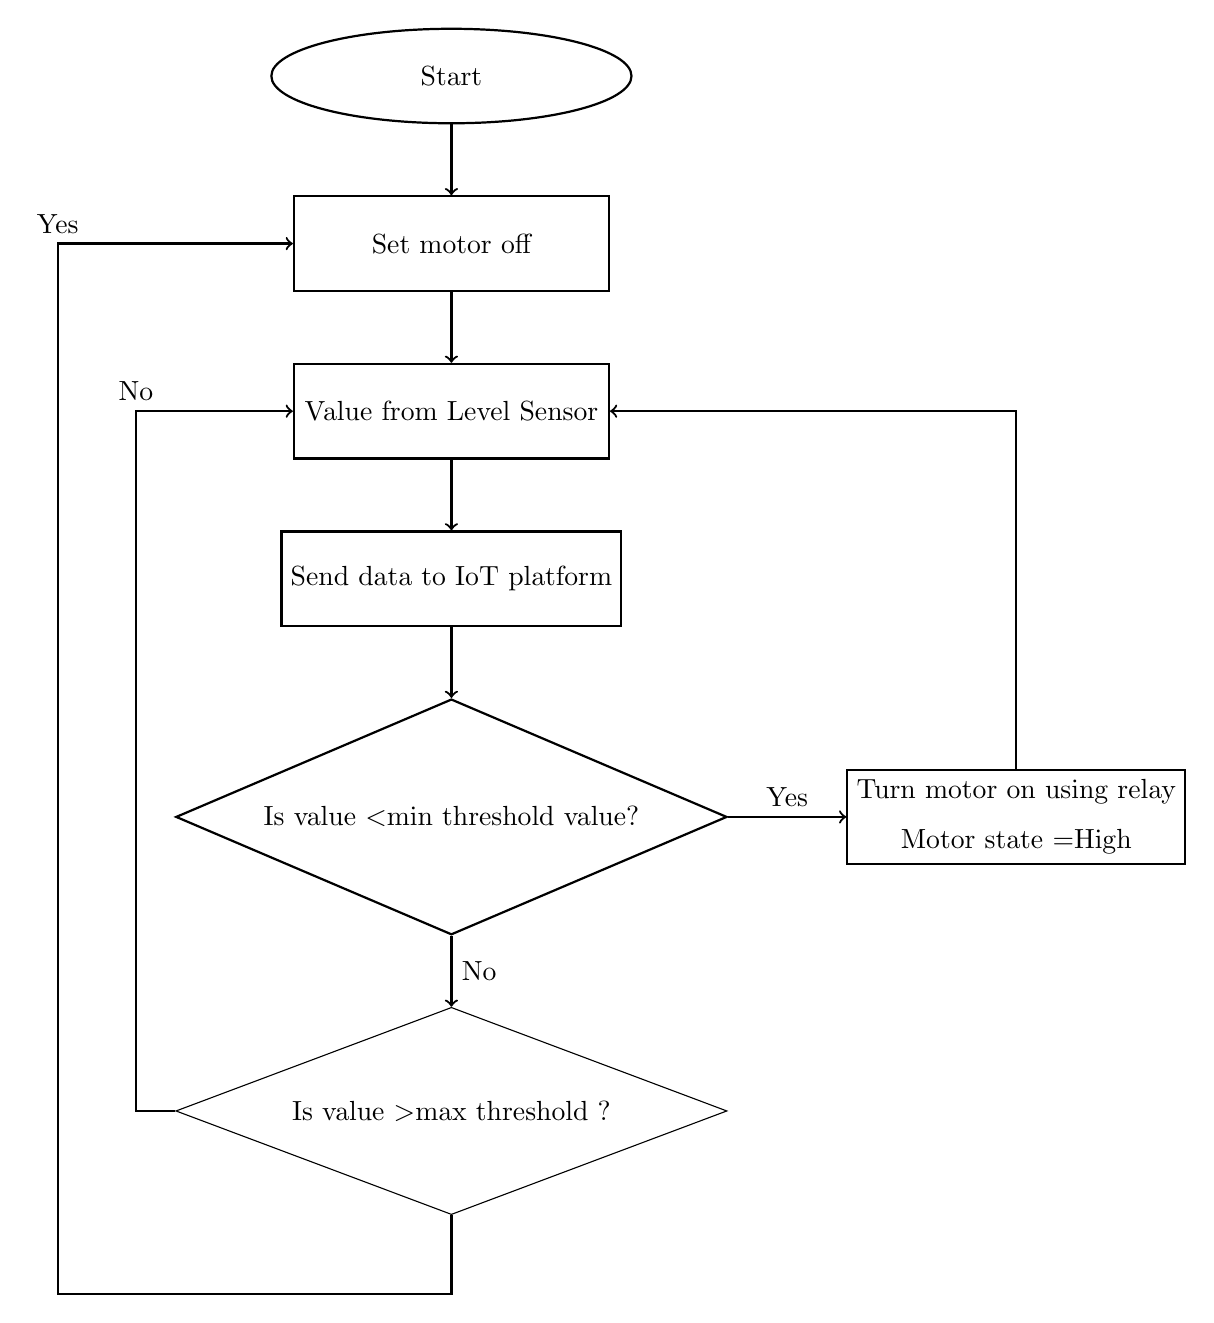
\begin{tikzpicture}  [node distance=0.9cm]
			\node[startstop,  thick] (start){Start};
			
			\node[process1, below=of start,  thick] (proc1) {Set motor off };
			\node[process1, below=of proc1,  thick] (proc2) {Value from Level Sensor  };
			\node [process1, below=of proc2 ,thick] (cloud) {Send data to IoT platform};
			\node[decision, below= of cloud,  thick] (dec1){Is value \textless   min threshold value?};
			\node[process1,  thick,right= 1.5cm of dec1, align=center] (proc3){Turn motor on using relay \\ Motor state =High};
			\node[decision,  below = of dec1,] (dec2){Is value  \textgreater max threshold ?};
			
			
			
			%arrow
			\draw [->,  thick] (start) -- (proc1);
			\draw [->,  thick] (proc1) -- (proc2);
			\draw [->,  thick] (proc2) -- (cloud);
			\draw [->,  thick] (cloud) --  (dec1);
			\draw [->,  thick] (dec1) --  node[anchor=west] {No}  (dec2);
			\draw [->,  thick] (dec1) -- node[anchor=south] {Yes} (proc3);
			\draw [->,  thick] (proc3.north) |-  (proc2.east);
			\draw[->,  thick] (dec2.west) -- ++ (-0.5,0)  |- node[anchor=south] {No}  (proc2.west);
			\draw[->,  thick] (dec2.south) -- ++ (0,-1) -- ++(-5,0) |- node[anchor=south] {Yes}  (proc1.west);
			
			%	
		\end{tikzpicture}
		
	\end{center}
	\begin{figure}[ht]
		
		\captionsetup{font=large}
		\caption{ Flowchart of water level sensor}
		
	\end{figure}
	
	
	%----------------------------------------------------- FLowchart: Light Automation
	
	
	
	
	% ------------------------------------------------------------------
	\pagebreak
	\subsection{Flowchart of PIR sensor with LDR  for Light Automation}
	
	\vspace{10 px}
	\begin{center}
		
		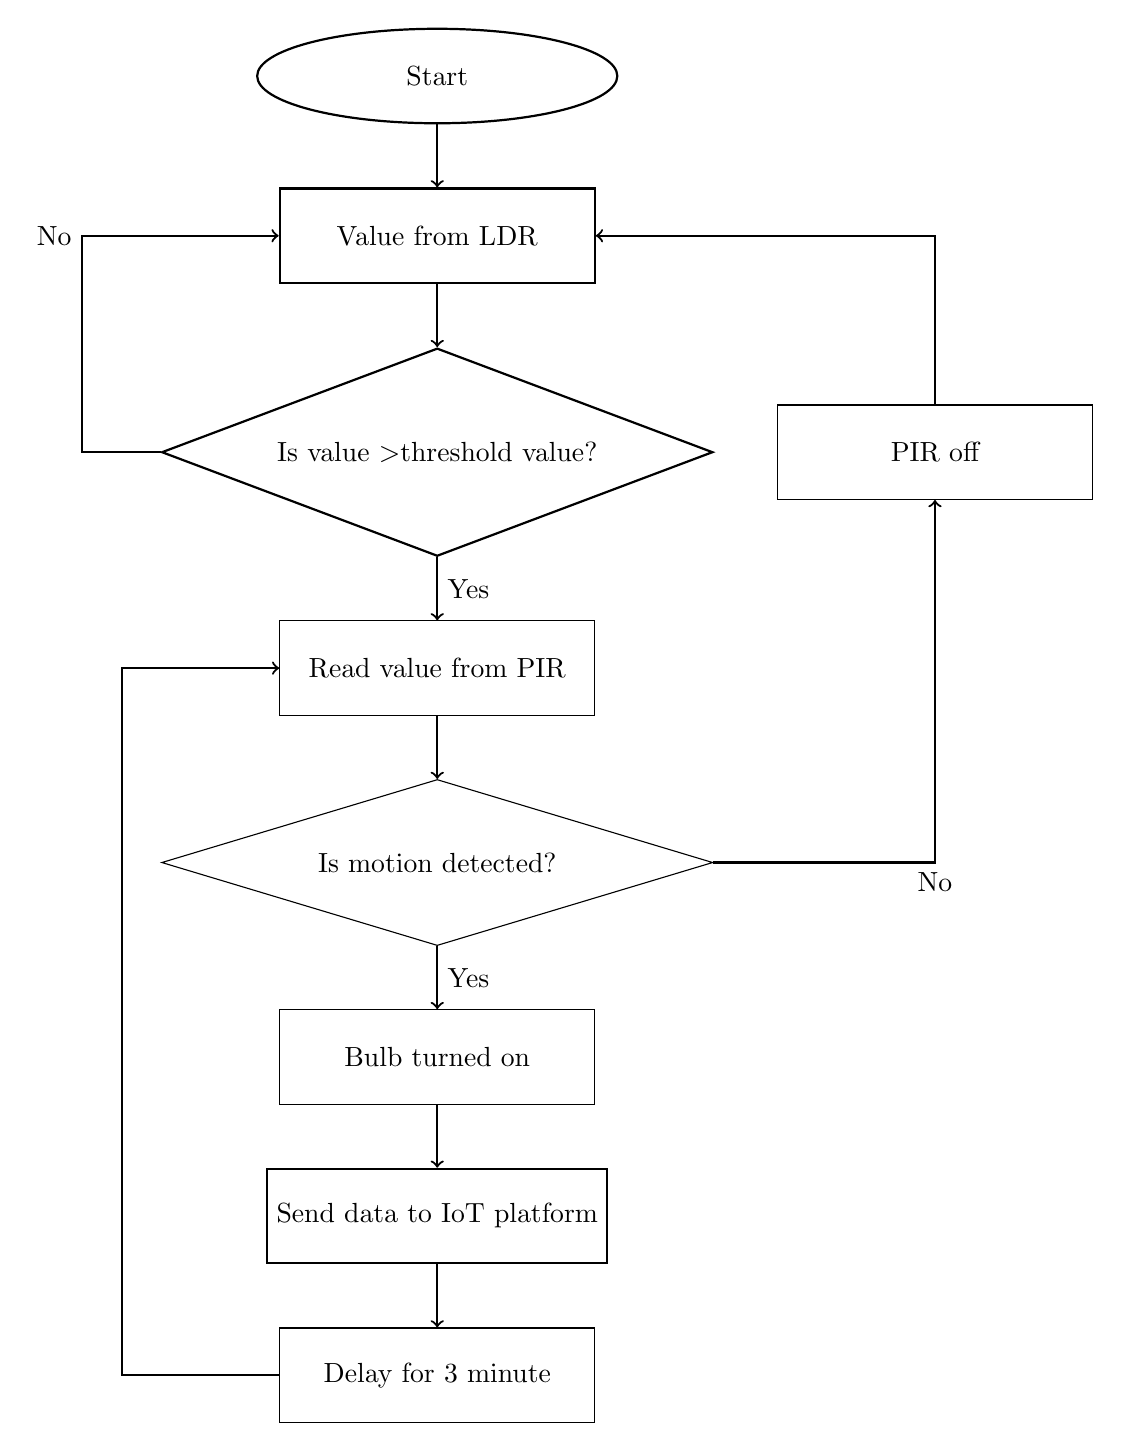
\begin{tikzpicture}  [node distance=0.8cm]
			\node[startstop,  thick] (start){Start};
			\node[process1, below=of start,  thick] (proc1) {Value from LDR };
			
			\node[decision, below=of proc1,  thick] (dec1){Is value \textgreater  threshold value?};
			%	\node[process1, below=of dec1] (proc2){PIR sensor turned on};
			\node[process1, below=of dec1] (proc3){Read value from PIR};
			\node[decision, below=of proc3] (dec2) {Is motion detected?};
			\node[process1, below=of dec2,align=center] (proc4) {Bulb turned on};	
			\node [process1, below=of proc4 ,thick] (cloud) {Send data to IoT platform};
			\node[process1, below=of cloud] (proc5) {Delay for 3 minute};
			\node[process1,right=of dec1](proc6){PIR off};
			
			
			
			%arrow
			\draw [->,  thick] (start) -- (proc1);
			\draw [->,  thick] (proc1) -- (dec1);
			
			\draw [->,  thick] (dec1) -- node[anchor=west]{Yes} (proc3);
			%	\draw [->,  thick] (proc2) -- (proc3);
			\draw [->,  thick] (proc3) -- (dec2);
			\draw [->,  thick] (dec2) -- node[anchor=west]{Yes} (proc4);
			\draw [->,  thick] (cloud) -- (proc5);
			\draw [->,  thick] (proc4) -- (cloud);
			\draw [->,  thick] (proc5.west) -- ++(-2,0) |- (proc3.west);
			\draw [->,  thick] (dec2.east) -| node[anchor=north]{No} (proc6.south);
			\draw [->,  thick] (proc6.north) |- (proc1.east);
			\draw [->,  thick] (dec1.west) --  ++(-1,0) |-  node[anchor=east]{No} (proc1.west);
			
		\end{tikzpicture}
		
	\end{center}
	\begin{figure}[ht]
		
		\captionsetup{font=large}
		\caption{ Flowchart of PIR sensor with LDR}
		
	\end{figure}
	
	
	
	%----------------------------------------------------- FLowchart: Door Automation ------------------------------------------------------------------
	\pagebreak
	\subsection{Flowchart of RFID  for Door Automation}
	\vspace{10 px};
	\begin{center}
		
		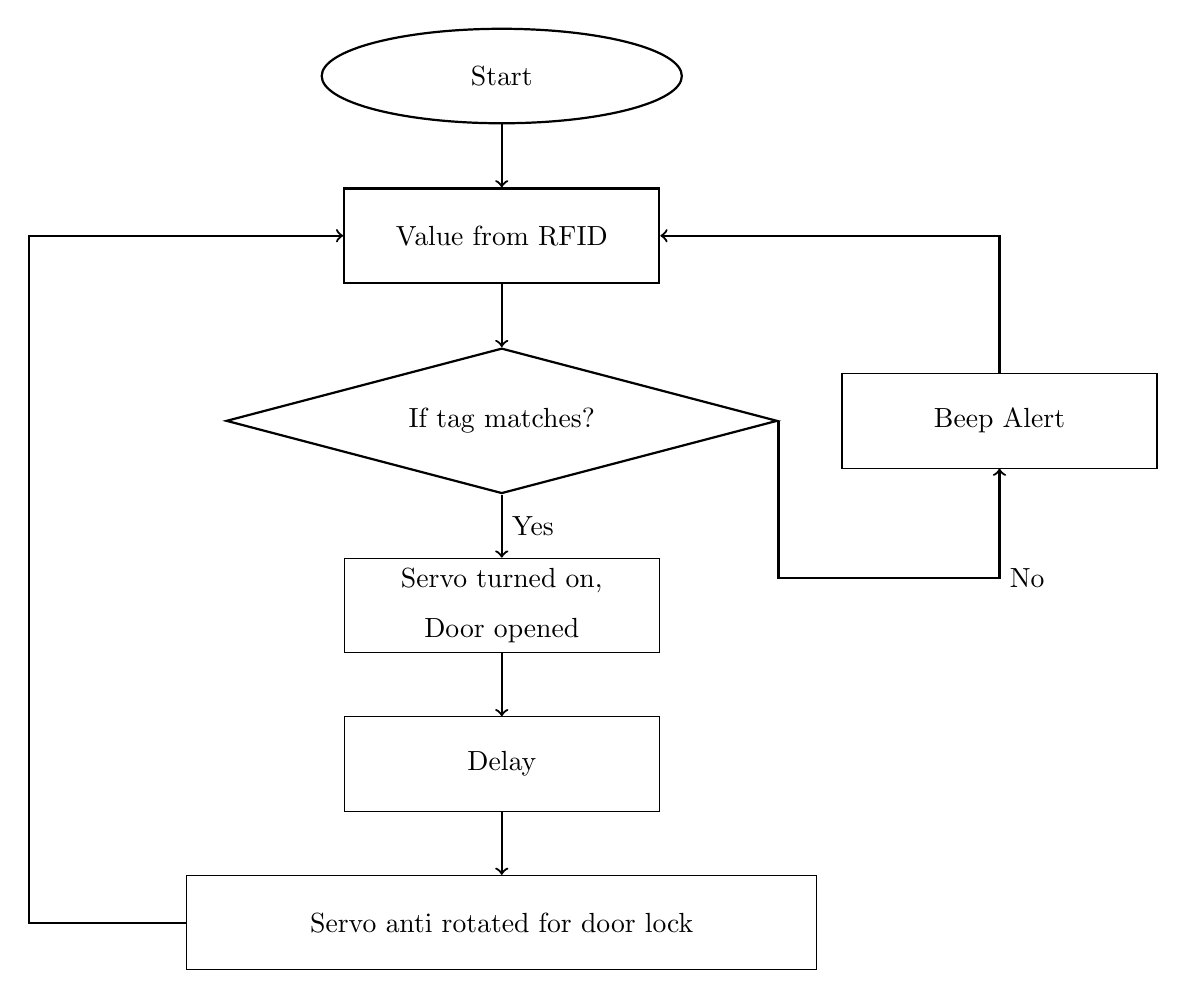
\begin{tikzpicture}  [node distance=0.8cm]
			\node[startstop,  thick] (start){Start};
		%	\node[process1, below=of start,  thick] (proc11) {count = 0 };
		%	\node[decision, below=of proc11,  thick] (dec2){If count less than 3  ?};
			\node[process1, below=of start,  thick] (proc1) {Value from RFID };
			\node[decision, below=of proc1,  thick] (dec1){If tag matches?};
			\node[process1, below=of dec1, align=center] (proc2){ Servo turned on, \\ Door opened };
			\node[process1, below=of proc2] (proc3){Delay};
			\node[process, below=of proc3] (proc4) {Servo anti rotated for door lock};
			\node[process1, right=of dec1 , align=center] (proc5){Beep Alert};
		%	\node[startstop,below=of proc4] (stop){stop};
		%	\node[process1, left=of proc1] (proc12) { Send alert to the owner};
		%	\node[process1, left= of proc2,  thick] (proc13) {Lock door for 3 minute };
			
			
			%arrow
			\draw [->,  thick] (start) -- (proc1);
			
		%	\draw [->,  thick] (proc11) -- (dec2);
		%	\draw [->,  thick] (dec2) --node [anchor=west]{Yes} (proc1);
			\draw [->,  thick] (proc1) -- (dec1);
			\draw [->,  thick] (dec1) -- node[anchor=west]{Yes} (proc2);
			\draw [->,  thick] (proc2) -- (proc3);
			\draw [->,  thick] (dec1.east)-- ++(0,-2)-- ++(2,0) -|  node[anchor=west]{No} (proc5.south);
			\draw [->,  thick] (proc3) -- (proc4);
		%	\draw [->,  thick] (proc12) -- (proc13);
		%	\draw [->,  thick] (proc13.west) -- ++(-1,0)  |-(proc11.west);
			\draw [->,  thick] (proc4.west) -- ++(-2,0) |- (proc1.west);
			\draw [->,  thick] (proc5.north) |- (proc1);
		%	\draw [->,  thick] (dec1) -- node[anchor=south]{No} (proc5);
			
			
			
		\end{tikzpicture}
		
	\end{center}
	\begin{figure}[ht]
		
		\captionsetup{font=large}
		\caption{Flowchart of RFID for door automation }
		
	\end{figure}
	
	%------------------------------------FLowchart of Blynkkk -------------------------
	%	\pagebreak
	%	\subsection{Flowchart of Blynk App or Website }
	%	\begin{justify}
		%		In the below flowchart, we update data from or to Blynk Cloud to our Blynk website or app. We display all the ongoing data into our app. If   system is switched to manually operating mode, the we can control light operation from the app.  
		%	\end{justify}
	
	%	\begin{center}
		
		%		\begin{tikzpicture}  [node distance=1cm]
			%			\node[startstop,  thick] (start){Start};
			%			\node[process1, below=of start,  thick] (proc1) {Update data from or to  Blynk Cloud};
			%			\node[process1, below=of proc1,  thick] (proc2){Display data from the Home};
			
			%			\node[decision, below  = of proc2,  thick, align=center] (dec1) {If system is in manual mode? };
			%			\node[process1, below = of dec1,  thick, align=center] (proc4){Control Home Functions   };
			
			
			%arrow
			%			\draw [->,  thick] (start) -- (proc1);
			%			\draw [->,  thick] (proc1) -- (proc2);
			%			\draw [->,  thick] (proc2) -- (dec1);
			%\draw [->,  thick] (proc3) -- (dec1);
			%			\draw [->,  thick] (dec1.west)  -- ++(-1,0) node[anchor=east] {No} |- (proc1.west);
			%			\draw [->,  thick] (dec1)  -- node[anchor=west] {Yes} (proc4);
			
			%			\draw [->,  thick] (proc4.east) -- ++(1.5,0)  |- (proc1.east);
			%		\end{tikzpicture}
		
		%	\end{center}
	%	\begin{figure}[ht]
		
		
		%		\caption{Flowchart of Blynk App or Website}
		
		%	\end{figure}
	
	
	
	
	%----------------------------------------------EPILOUGE-----------------------------
	\chapter{RESULT AND DISCUSSION}
	
	\section{Output}
	\begin{justify}

	The proposed Home Automation system has been achieved. In this system, we incorporate different sensors to control and monitor home appliances. All the sensors used is tested and calibrated properly to ensure proper execution.  MQ2 sensor, PIR, LDR, RFID, and Water level sensor is used in this project. We have successfully controlled the home appliances automatically which can also be controlled and monitored from Arduino IoT platform. 
	\end{justify}
	\section{Limitations}
	\begin{justify}
		

	Since the device is designed as a prototype and made using the simple electronic components, there are some limitations that are listed below:\\
	1. This project home automation does not operate during power interruptions and totally rely on availablity of electricity.\\
	2.  The reliability of our project heavily depends on a stable and robust internet connection. Network outages or disruptions affect the functionality of IoT devices.\\
	3. Since,  water level sensor is  of prototyping standard, it lacks the flexibility to adapt to various shapes and sizes of water tanks commonly installed in homes.\\
	4. Though it is a fully automatic system, it cannot be controlled using manual switches. \\
	
			\end{justify}
	%--------------------Schedule ----------------------
	\section{Schedule}
	

		
		
		%\begin{table}[h]
			
			%\centering
			
			%\caption{Work Schedule}
			%\vspace{7 px}
			%\renewcommand{\arraystretch}{2}
			%\arrayrulecolor{gray}
			%\setlength{\arrayrulewidth}{1.5pt} % Adjust line thickness
			%\begin{tabular}{|l|p{1.2cm}|p{1.2cm}|p{1.2cm}|p{1.2cm}|p{1.2cm}|p{1.2cm}|}
				%\hline
				%\multirow{2}{*}{Activities} & \multicolumn{6}{c|}{Months} \\
				%\cline{2-7}
				%& First & Second &Third &Fourth & Fifth & Sixth \\
				%\hline
				%Research &\cellcolor{black} &\cellcolor{black} &\cellcolor{black} &\cellcolor{black} & & %\\ \hline
				%System Design & & \cellcolor{black}   &\cellcolor{black} & & &\\ \hline
				
				
				%Hardware Collection & & &  \cellcolor{black} & \cellcolor{black}& & \\ \hline
				
				%Coding               &  & & &\cellcolor{black} &\cellcolor{black} & \\ \hline
				%Interfacing Hardware & & & &\cellcolor{black} &\cellcolor{black} & \cellcolor{black} \\ %\hline
				%Documentation & & \cellcolor{black}& \cellcolor{black}& \cellcolor{black}& %\cellcolor{black}&\cellcolor{black} \\ \hline
				
		%	\end{tabular}
			
			
			
			
			
			
			
		%\end{table}
		
		
		\begin{center}
			
		\vspace{10 px}
	\begin{ganttchart}[
		hgrid,
		vgrid,
		x unit=0.9cm,
		y unit title=1cm,
		y unit chart=1.5cm,
		title height=1,
		title label font=\bfseries\footnotesize,
		bar height=0.5,
		bar label font=\small,
		group label font=\small,
		milestone label font=\small,
		milestone height=0.8,
		group height=1cm,
		bar/.append style={fill=blue!30},
		]{1}{12}
		\gantttitle{Months}{12} \\
		\gantttitle{July}{2}
		\gantttitle{August}{2}
		\gantttitle{November}{2}
		\gantttitle{December}{2}
		\gantttitle{January}{2}
		\gantttitle{February}{2}\\
	   	\ganttbar{Research}{1}{6} \\
		\ganttbar{System Design}{3}{6} \\
		\ganttbar{Hardware Collection} {5}{8}\\
		\ganttbar{Coding}{7}{10} \\
		\ganttbar{Interfacing Hardware}{8}{11} \\
		\ganttbar{Documentation}{2}{12} 
	\end{ganttchart}
		
			\begin{figure}[ht]
			
			\captionsetup{font=large}
			\caption{Gantt Chart}
			
		\end{figure}
	\end{center}
		
	
	
	
	
	
	%-----------------COst Estimation- ----------------
	\newpage
	\section{Cost Estimation}

	\begin{center}
		
		\begin{table}[h]
			
			\centering
				
			\caption{Budget Analysis}
			\vspace{7 px}
			\renewcommand{\arraystretch}{2}
			\arrayrulecolor{gray}
			\setlength{\arrayrulewidth}{1.5pt} % Adjust line thickness
			\begin{tabular}{|c|c|c|c|}
			\hline
			\textbf{Equipments} &	\textbf{Quantity} & 	\textbf{Unit Price}& 	\textbf{Total (Rs.) }\\
			\hline
			ESP32 & 1 & 1250 & 1250 \\
			\hline
			Water level sensor & 1 & 200 & 200 \\
			\hline
			Relay single channel & 6 & 160 & 960 \\
			\hline
			12V DC Fan & 1 & 280 & 280 \\
			\hline
			RFID-RC522 module & 1 & 950 & 950 \\
			\hline
			Buzzer & 2 & 60 & 120 \\
			\hline
			Transistor BC 547 & 6 & 10 & 60\\
			\hline
			Servo Motor& 2 & 400 & 800 \\
			\hline
			LDR & 5 & 25 & 125\\
			\hline
			PIR sensor & 4& 300& 1200\\
			\hline
			MQ2 Sensor&1 & 300&300 \\
			\hline
			Water Pump Motor & 1 & 200 & 200\\
			\hline
			\multicolumn{3}{|c|}{ \textbf{Total} } & 6445 \\
			\hline
			
			
		\end{tabular}
		
			
			
			
			
			
			
		\end{table}
		
		
		
		
		
		
		
		
	\end{center}
	
	

	
	%---------------------CONCLUSION and FUTURE enhancements
	
	\chapter{CONCLUSION AND FUTURE ENHANCEMENT}
	
	
	\section{Conclusion}
	
	\begin{justify}
		

   
    
    	With the help of ESP32 and  IoT concept, home automation has been acheived. The data from  sensor is sent to micro controller ESP32. On receiving data, the ESP32 facilitates relay to control switches and fan, buzzer according to the logic used. ESP32 also continuously send data to the cloud and  home appliances can be controlled and monitor through IoT platform. \\
    Five different sensors are used to control home automation; MQ2 sensor, RFID, PIR, LDR and water level sensor.\\
    MQ2 sensor is used for Kitchen Fire Protection. When harmful gases is detected, ESP32 sends signal to turn on exit fan, turn off regulator using servo motor and turn on emergency beep and cut off power supply of kitchen room. Amount of gases can be constantly monitored from IOT cloud platform.\\
    Water sensor is used for Tank Water Management. Water level sensor senses the level of water in tank. When tank is around full, water is not pumped into tank and when water level of tank falls down, water is automatically pumped into tank without spillage of water by sending signal from ESP32. Relay module is used to drive water pump motor. Level of water in tank can also be monitored from IoT platform and also can control water pump motor using IoT platform.\\
    PIR along with LDR  is used for Light Control.  We use PIR sensor with LDR sensor to work PIR only on night time. The value of PIR is send to ESP32 and ESP32 sends control signal to turn off or on room light. Light of each room can also be controlled from IoT platform.\\ 
    RFID sensor is use for door automation. It is also connected to ESP32. If the tag matches the RFID reader the door gets open. If the tag doesn't matches the door won't get opened. Door lock can also be controlled from IoT platform.
	
		\end{justify}
	%------------------------------Future enhancement---------------------
	\section{Future Enhancement}
		\begin{justify}
Due to various factors like limited time, failure of devices, we are not able to give our full attention to all the sectors of project and concerned only towards our main objectives. When considering ways to enhance and make our home project more smart in future, there are numerous  possibilities for additions:\\
		1. Power Backup Solutions: Implement a  power backup system, to ensure uninterrupted functionality during power outages.\\
		2. Smart Perimeter Security: Integrate smart sensors along the fence and home boundary to detect unauthorized entry attempts.\\
		3.Versatile Water Level Sensor Design: Develop an adaptable water level sensor that can accommodate large water tanks commonly installed in homes.
	
		
		
	\end{justify}

		
		
		
		

	
	
	
	
	%-------------------------------------------------References----------------------------
	
	
	
	
	\justifying
	\printbibliography[title={REFERENCES}]
	
	\addcontentsline {toc} {chapter} {References}	
	%	\printbibliography
	
	%	\bibliographystyle{ieeetran}
	
	
	
	
	
	
	% Annex

	
	
\end{document}







